\chapter{METHODOLOGY}
\section{Modifying the Testing Framework}
The framework of the study is divided into two parts. First, we expanded the QoS Testing Framework (hereby referred to as the \textit{Framework}) from Regencia and Yu to support different classes of topologies: fat-tree topologies with fanout greater than 2, some typical topology shapes, general graphs, and data from the Internet Topology Zoo that follow the constraints in section 1.5. Second, we simulate artificial network load with the same methodology as the Regencia and Yu study onto the newly implemented topologies with the same queue management algorithms. 

To accomplish this, we modified the way the \textit{topology configuration} file is read in the Framework. In the original Framework, the topology configuration file contains information about the number of clients and the number of layers in a tree topology, which is then used by each of the \textit{configuration generator} files to reconstruct the topology within itself to generate the correct configuration (Figure \ref{fig:original_architecture}). 

We modifed the Framework such that an intermediary script called the \textit{Topology Information Generator} contains the implementation of the topology (Figure \ref{fig:new_architecture}). The Topology Information Generator emitted a GraphML file that could be read by the configuration generators to generate the necessary configuration files. For typical topologies such as the fat-tree and mesh, the \textsc{NetworkX} functions \textsc{balanced\_tree} and \textsc{complete\_graph} functions were used.. For topologies from the Internet Topology Zoo data, the generator parsed the corresponding GraphML file from the ITZ with the \textsc{NetworkX} library to generate the same information file.

\begin{figure}[htbp!]
    \centering
    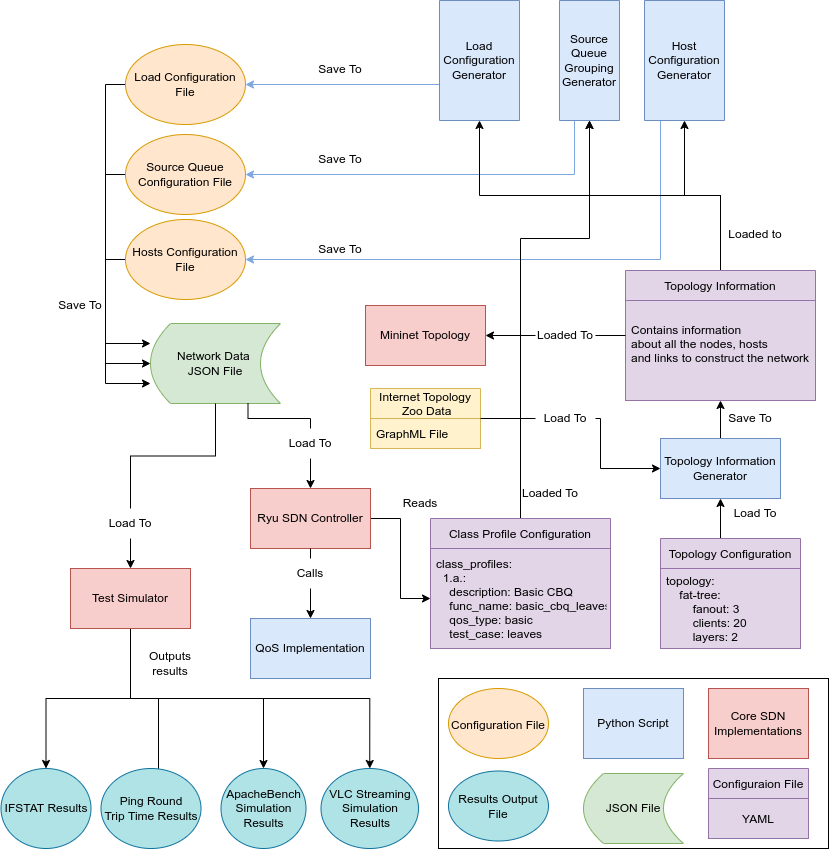
\includegraphics[width=\textwidth]{Figures/Test Framework Architecture.drawio.png}
    \caption{The architecture of the Modified QoS Testing Framework}
    \label{fig:new_architecture}
\end{figure}

The framework was further modified so that the Ryu Controller script now uses the STP protocol to decide the paths of the packets in the topologies, since typical topologies like the mesh and real-life data from the ITZ contain loops for better network resiliency \cite{smith_shortest_2011}. The reference \textsc{simple\_switch\_stp\_13.py} code from the Ryu Library is used as a basis to develop the controller that will run on any topology and with any QoS queue management technique.

Finally, we simplified the framework so that the framework no longer needs pickle files to specify the QoS Implementations. Instead, the Ryu Controller directly calls the appropriate QoS Implementation according to the algorithm specified by the \textit{Class Profile Configuration} file. The modified framework is installed on a system configured as described in Figure \ref{fig:tools}. Software in the \textit{SDN Simulation} column were used for simulating the networks and running the tests, while the tools in the \textit{Topology Processing} column were used for selecting, diagramming, and processing the various topologies.

\begin{figure}[htbp]
    \centering
    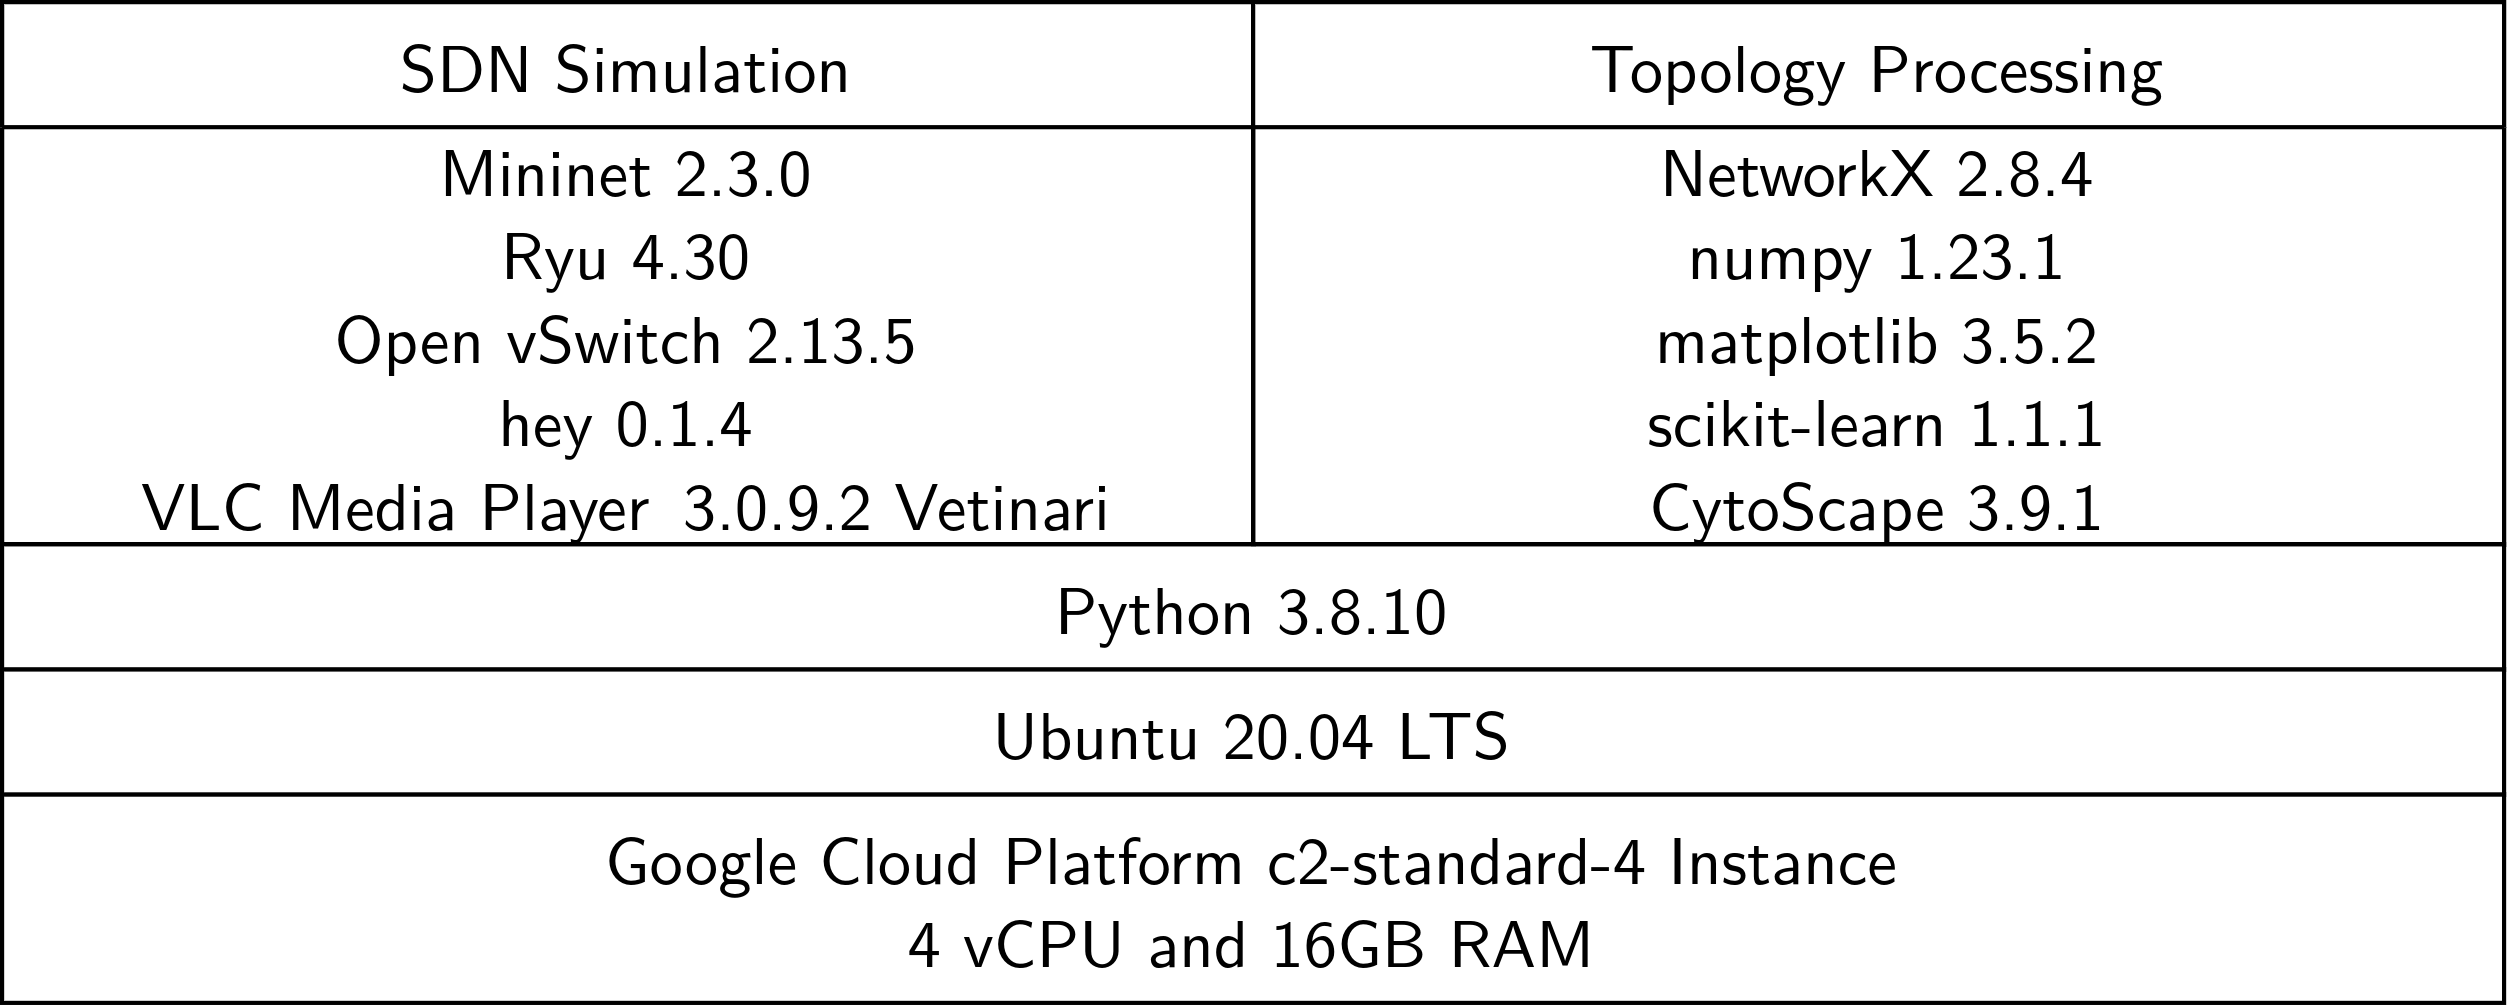
\includegraphics[width=\textwidth]{Figures/Test Machine Configuration.drawio.png}
    \caption{The machine configuration and software tools used in the experiment}
    \label{fig:tools}
\end{figure}

\section{Selection of Networks for Testing} \label{sec:selection}
We tested the following topologies:
\begin{enumerate}
    \item Complete Mesh topology with 5 vertices in the mesh (Figure \ref{fig:CompleteMesh})
    \item Fat-tree topology with two layers and fan-out 3 (Figure \ref{fig:BalancedTree})
    \item Topology from the Internet Topology Zoo, Regional or Country data with less than 40 nodes
\end{enumerate}

The choice of topologies from the Internet Topology Zoo was based on two features: the number of nodes and the number of edges (links) in the graph. From the dataset in the ITZ, there were 133 topologies that are either regional or country data that at most 40 nodes. This limit is due to the limited resources of the machine that runs the simulations. We first clustered the topologies according to the number of nodes and edges to ensure that a variety of networks that are representative of the dataset is chosen. The clustering was done by reading all 133 topologies into the NetworkX library, extracting the number of nodes and edges, and using the \textsc{scikit-learn} K-Means clustering library \cite{pedregosa_scikit-learn_2011}. All default settings for the scikit-learn implementation of K-Means Clustering was used, except for the number of clusters set at $4$. Each node-edge data point was given the same weight. The Python code for this procedure is shown in Listing 1. Then, 10 random topologies were chosen from the four clusters with NumPy, proportional to the number of topologies in each group. The list of the chosen topologies are shown in Table \ref{tab:choices} in Chapter 4.

\section{Topology Configuration} \label{sec:topo_config}
To implement the topologies within the context of the simulations, we modified the fat-tree topology from the original study by Regencia and Yu by changing the number, arrangement, and links in the switches that connect the ``core'' switch to the clients. The ``core'' switch is the switch that connects to a switch connecting all servers in a star topology formation. The topology to be changed corresponds to the circled switches in Figure \ref{fig:original_topology}.

\begin{figure}[htbp]
    \centering
    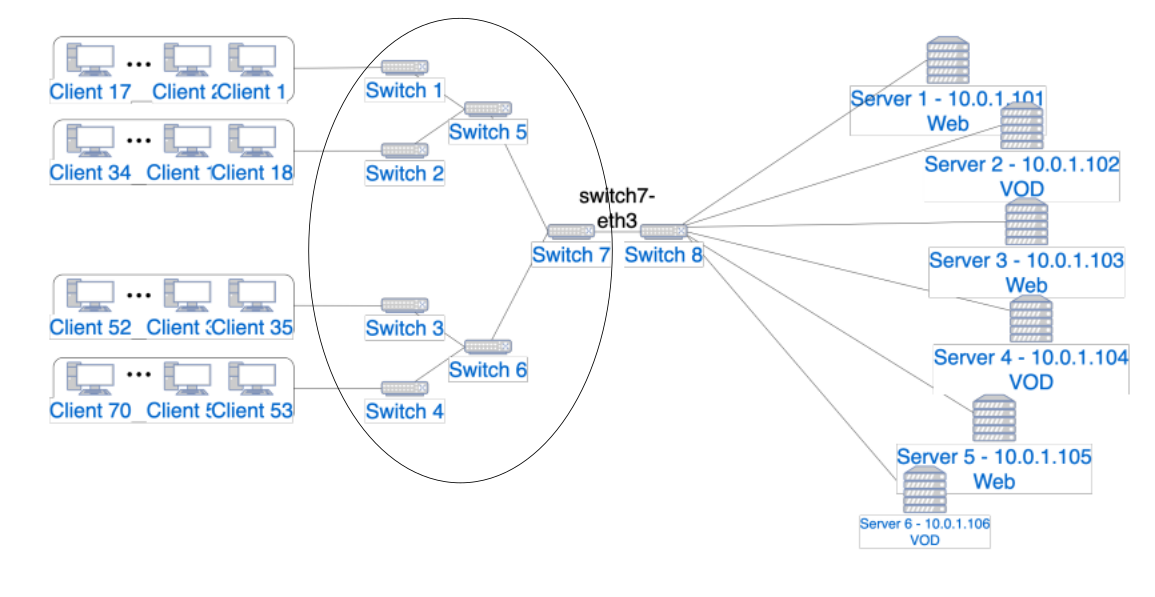
\includegraphics[width=\textwidth]{Figures/original_topology.png}
    \caption{Diagram of a fat-tree topology tested in Regencia and Yu}
    \label{fig:original_topology}
\end{figure}

The ``core'' switch in the fat-tree topology was still the root switch of the tree. In the complete mesh topology, the node with the numerical label $0$ is considered to be the root switch, since the topologies has at least one symmetry with respect to any node in the mesh. For the topologies from the Internet Topology Zoo, we simulate the worst case scenario by assigning the core as the node with the highest number of total hops from all other nodes, which is calculated with the Floyd-Warshall algorithm provided by the NetworkX library.

Clients were placed on all ``leaf'' switches, or switches furthest away from the ``core'' switch, which are switches that have the longest path from the core switch in the graph that represents the topology. As an exception, the fat-tree topology had clients connected to its explicit leaf switches. The clients will be distributed equally among the switches, that is, each switch will have at least $\lfloor\dfrac{n}{s} \rfloor$ and at most $\lfloor{\dfrac{n}{s}}\rfloor + 1$ clients, where $n$ is the number of clients and $s$ is the number of switches in the network. Finally, four servers were connected to the server switch to complete the topology. Network diagrams of the tested topologies are included in Appendix I.

Links were configured with their default setting of 10Gbps in Mininet, as in the previous study, since the data provided by the ITZ was not complete to simulate real-life link speeds.

\section{Server Configuration}
Two servers hosted a Python server from the http.server library, while two other servers hosted a VLC streaming server using the Real Time Streaming Protocol. Table \ref{tab:httpserverconfig} shows the files hosted by the HTTP servers, and Table \ref{tab:vlcconfig} shows the videos hosted by the VLC servers.

\begin{table}[htbp]
    \centering
    \begin{tabular}{cccc}
        \toprule
        \multirow{2}{*}{Server ID} & \multirow{2}{*}{Server IP Address} & \multicolumn{2}{c}{File Size and Type} \\
         &  & Low Load & High Load \\
        \midrule
        Server 1 & 10.0.1.101 & \qty{100}{\kilo \byte} JPEG & \qty{10}{\mega \byte} JPEG \\
        Server 3 & 10.0.1.103 & \qty{16}{\mega \byte} PDF & \qty{100}{\mega \byte} PDF  \\
        \bottomrule
    \end{tabular}
    \caption{Files hosted by the two Python http.server servers}
    \label{tab:httpserverconfig}
\end{table}

\begin{table}[htbp]
    \centering
    \begin{tabular}{cccc}
        \toprule
        \multirow{2}{*}{Server ID} & \multirow{2}{*}{Server IP Address} & \multicolumn{2}{c}{Video Resolution} \\
         &  & Low Load & High Load \\
        \midrule
        Server 2 & 10.0.1.102 & 360p & 480p \\
        Server 4 & 10.0.1.104 & 480p & 720p  \\
        \bottomrule
    \end{tabular}
    \caption{Files hosted by the two VLC RTSP servers}
    \label{tab:vlcconfig}
\end{table}

\section{Client Configuration}
48 clients simultaneously ran a \textsc{hey} HTTP benchmark test instance and a VLC client instance. Each client will request for different files from the server, and every file in each server will get requests as equally as possible. Table \ref{tab:clientconfig} shows the configuration of these clients.

\begin{table}[htbp]
    \centering
    \begin{tabular}{ccc}
    \toprule
        Client numbers & Server & Load\\
    \midrule
        \multirow{2}{*}{$1, 5, 9, 13, \dots 41, 45$}  & Server 1 & Low \\
        & Server 2 & Low \\ \hline
        \multirow{2}{*}{$2, 6, 10, 14, \dots 42, 46$}  & Server 3 & Low \\
        & Server 4 & Low \\ \hline
        \multirow{2}{*}{$3, 7, 11, 15, \dots 43, 47$}  & Server 1 & High \\
        & Server 2 & High \\ \hline
        \multirow{2}{*}{$4, 8, 12, 16, \dots 44, 48$}  & Server 3 & High \\
        & Server 4 & High \\
    \bottomrule
    \end{tabular}
    \caption{Configurations for clients denoting the server and the load that the client will request in the simulations}
    \label{tab:clientconfig}
\end{table}

\section{Quality of Service configuration}
In this experiment, two quality of service algorithms were tested: Basic CBQ and Source CBQ, all implemented in the leaves. The parameters found in Tables \ref{tab:CBQconfig} (Basic CBQ) and \ref{tab:SBQconfig} (Source CBQ) were applied to all ports of switches that were connected to clients with the \textsc{ovs-ofctl} command.

\begin{table}[htbp]
    \centering
    \begin{tabular}{ccccc}
    \toprule
        Queue number & Traffic Protocol & Application & Maximum bandwidth & Priority\\
    \midrule
        $Q_0$ & TCP & HTTP traffic & \qty{333.33}{\mega \bit / \second} & 1 \\
        $Q_1$ & UDP & Video streaming & \qty{333.33}{\mega \bit / \second} & 2 \\
        $Q_2$ & ICMP, ARP & Network control & \qty{333.33}{\mega \bit / \second} & 0 \\
    \bottomrule
    \end{tabular}
    \caption{QoS configuration used to implement simple CBQ QoS enforcement}
    \label{tab:CBQconfig}
\end{table}

\begin{table}[htbp]
    \centering
    \begin{tabular}{cccc}
    \toprule
        Queue number & Source & \makecell{Minimum and \\Maximum bandwidth} & Priority\\
    \midrule
        $Q_0$ & 10.0.0.1, 4, 7 ... & \qty{333.33}{\mega \bit / \second} & 1 \\
        $Q_1$ & 10.0.0.2, 5, 8 ... & \qty{333.33}{\mega \bit / \second} & 2 \\
        $Q_2$ & 10.0.0.3, 6, 9 ... & \qty{333.33}{\mega \bit / \second} & 0 \\
    \bottomrule
    \end{tabular}
    \caption{QoS configuration used to implement Source-based CBQ QoS enforcement}
    \label{tab:SBQconfig}
\end{table}

\section{Network Simulation and Testing} \label{3:testing}
The methodology of testing the networks was similar to Chato and Yu \cite{chato_exploration_2016}, which was also used in Regencia and Yu \cite{yang_introducing_2022}. Since the modified framework uses STP, we had to wait for the STP to converge before running the rest of the tests. We waited for 60 seconds, which was empirically found to be enough STP to converge in all cases.

One key difference between this methodology and the methodology from Regencia and Yu is that different topologies take different amounts of time for the switches in the network to install flows. We define the \textit{convergence time} as the time it takes for pings to go consistently under 1 second after the STP established proper connections between the servers and the clients. Yoo and Yu have shown that the convergence time is different for different types of topologies \cite{yoo_building_2022}. Therefore, this characteristic is measured first before running other tests.

For every topology, the procedure described in Figure \ref{fig:benchmark} is followed.

\begin{figure}
    \centering
    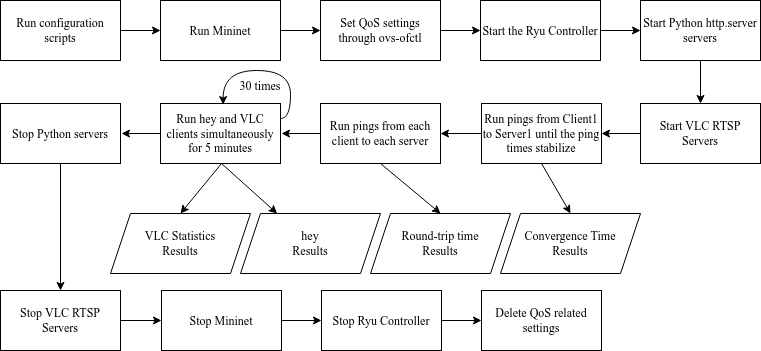
\includegraphics[width=\textwidth]{Figures/Test Procedure.drawio.png}
    \caption{The procedure for running the benchmarks}
    \label{fig:benchmark}
\end{figure}

First, the tested network is loaded into Python with the NetworkX library. Then, the network is modified to include the four servers and 48 clients. The modified NetworkX object is sent to the \textit{configuration generator}. The configuration generator generates the necessary configuration files. Then, Mininet was initialized with the NetworkX object, which initialized all the switches and hosts in of the experimental setup. The QoS configuration script, which was generated by the configuration generator, was applied afterwards. Next, the Ryu controller was started, followed by the Python http servers and the VLC servers. Then, the command \textsc{client1 ping -c 50 server1} was run to test for the convergence time. After that was completed, \textsc{ping} commands were executed from every client to every server for 20 times for the ping benchmark. Then, the VLC clients and textsc{hey} clients were started to perform the Video Streaming and HTTP benchmarks. The two aforementioned benchmarks were performed 30 times. It is important that the video streaming and HTTP benchmarks are performed after the round-trip time benchmark to ensure that the flows in the network are properly installed and the network has converged into a stable state.

